\documentclass[aps, prc, reprint]{revtex4-1}

\usepackage{amsmath}
\usepackage{mathtools}
\usepackage{amsfonts}
\usepackage{url}
\usepackage{xspace}
\usepackage{siunitx}
\usepackage[usenames,dvipsnames]{xcolor}
\usepackage{float}
\usepackage[caption=false]{subfig}
\usepackage{framed}

\frenchspacing

% Defined macros

\DeclareMathOperator{\csch}{csch}
\DeclareMathOperator{\sech}{sech}

\newcommand{\degree}[0]{\ensuremath{^\circ}\xspace}
\renewcommand{\implies}{\Rightarrow}
\newcommand{\eval}[1]{\ensuremath{\left<#1\right>}}
\newcommand{\ket}[1]{\ensuremath{\left| #1 \right>}}
\newcommand{\bra}[1]{\ensuremath{\left< #1 \right|}}
\newcommand{\mel}[3]{\ensuremath{\left<#1 \right|\! #2 \!\left| #3 \right>}}
\newcommand{\proj}[2]{\ensuremath{\left<#1 \middle| #2 \right>}}

\newcommand{\pmat}[1]{\ensuremath{\begin{pmatrix}#1\end{pmatrix}}}

\newcommand{\pder}[2]{\ensuremath{\frac{\partial #1}{\partial #2}}}
\newcommand{\ppder}[2]{\ensuremath{\frac{\partial^2 #1}{\partial #2^2}}}
\newcommand{\ppmder}[3]{\ensuremath{\frac{\partial^2 #1}{\partial #2 \partial #3}}}

\newcommand{\pderc}[3]{\ensuremath{\left( \frac{\partial #1}{\partial #2} \right)_{\!\!#3}}}
\newcommand{\ppmderc}[4]{\ensuremath{\left( \frac{\partial^2 #1}{\partial #2 \partial #3} \right)_{\!\!#4}}}

\newcommand{\nuc}[2]{\ensuremath{{}^{#1}\text{#2}}}

\newcommand{\fresco}[0]{\textsc{Fresco}\xspace}
\newcommand{\sfresco}[0]{\textsc{Sfresco}\xspace}


\begin{document}

\title{PHY 982 Homework 3: Transfer reactions}
\author{Josh Bradt}
\author{Chris Izzo}
\date{April 23, 2015}

\maketitle

\section{Introduction}

For this assignment, we chose to study the $\nuc{40}{Ca}\,(d,p)\,\nuc{41}{Ca}$ reaction at \SI{65.0}{MeV} and \SI{11.8}{MeV}. The lower of these two energies is just above the Coulomb barrier. The target nucleus \nuc{40}{Ca} is doubly magic (with a $0^+$ ground state), and it fills the \emph{sd}-shell completely for both protons and neutrons. Assuming that the neutron is transfered from the deuteron's $1^+$ bound state into the $7/2^-$ ground state of \nuc{41}{Ca}, it will occupy the $1f_{7/2}$ single-particle state, which is in the \emph{pf}-shell.

To calculate the differential cross-sections of the transfer reaction, we used \fresco. The potential binding the deuteron was modeled with a Gaussian as suggested in the assignment, and the interaction between the \nuc{40}{Ca} core and the transferred neutron was modeled with a Woods-Saxon potential with the default parameters specified in the assignment. In the high-energy case, we used global optical potentials from the RIPL database \footnote{\texttt{https://www-nds.iaea.org/RIPL-3/}} to represent the rest of the interactions. In the low energy case, however, the RIPL database did not have an acceptable potential, so we used a parameterization from Koning and Delaroche \cite{Koning2003}.

\section{High-energy results}

\begin{figure}[bt]
	\centering
	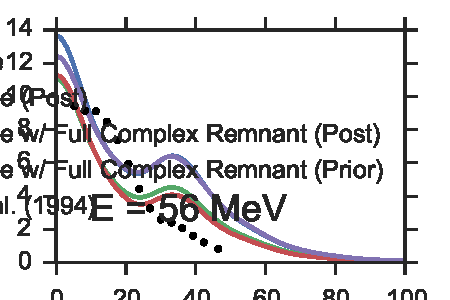
\includegraphics[width=\columnwidth]{{images/highen.pdf}}
	
	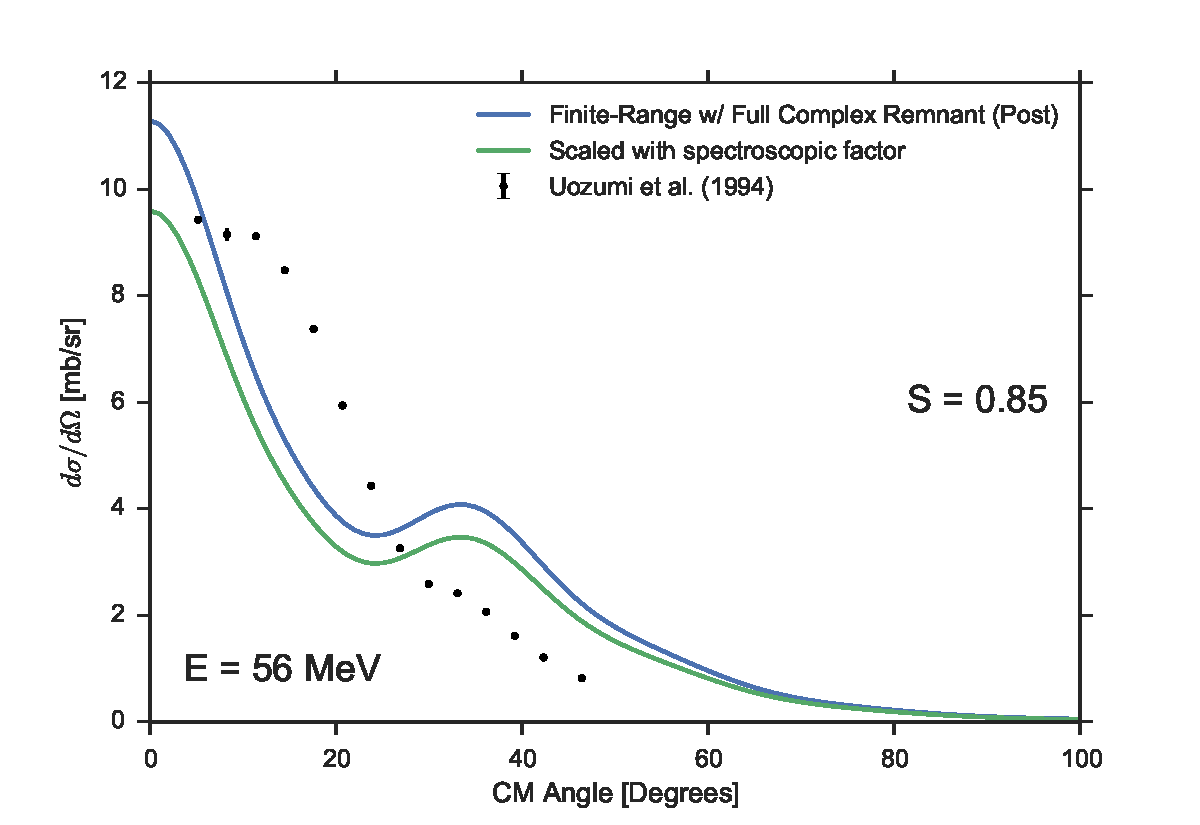
\includegraphics[width=\columnwidth]{{images/highen_sfactor.pdf}}
	\caption{The top graph shows the $\nuc{40}{Ca}\,(d,p)\,\nuc{41}{Ca}$ transfer cross sections at energy \SI{56}{MeV}. We assume that the neutron was transferred into the ground state of \nuc{41}{Ca}. The black points represent experimental cross sections from Uozumi et al. \cite{Uozumi1994}. The bottom plot shows a spectroscopic factor for the same data.}
	\label{fig:highen}
\end{figure}

Fig.~\ref{fig:highen} shows our results for the higher deuteron energy of \SI{56}{MeV}. The shape of the \fresco output is similar to the experimental data, but does not line up particularly well. This is likely due in part to the global optical potentials we used, but mainly due to the fact that DWBA is inherently an approximation, and may not have been the best choice in this regime.

We see that at this energy, the zero-range approximation gives results that are rather different from those of the finite-range approximation. The two post-form finite-range approximations give very similar results, but the prior-form result is quite different. This is not what we would expect since there should be no difference between the post and prior forms. (The fact that the post-form result is aligned with the zero-range result is entirely coincidental.) Therefore, this discrepancy must be a result of numerical errors, rather than some physical process.

The shape of the angular distribution makes sense when we consider the conservation of angular momentum.  The neutron is primarily in an s-wave when bound to the proton, but occupies an f-wave in the ground state of \nuc{41}{Ca}.  This requires a relatively large relative angular momentum between the projectile and target, corresponding to a large impact parameter.  For a large impact parameter, we expect to see the most scattering to forward angles, and less at backward angles.  This trend can be seen in the steady decrease of the angular cross section both in the experimental data and the \fresco output.

In the lower plot in Fig.~\ref{fig:highen}, we show our finite-range fit with a full complex remnant after scaling by a spectroscopic factor. This factor is defined as
\begin{equation}
	S^\text{exp} = \frac{\sigma^\text{exp}}{\sigma^\text{DWBA}}.
\end{equation}
We determined this factor to be $S^\text{exp} = 0.85$ by manually scaling the \fresco results until they agreed with the data points.

\begin{figure*}[t]
	\centering
	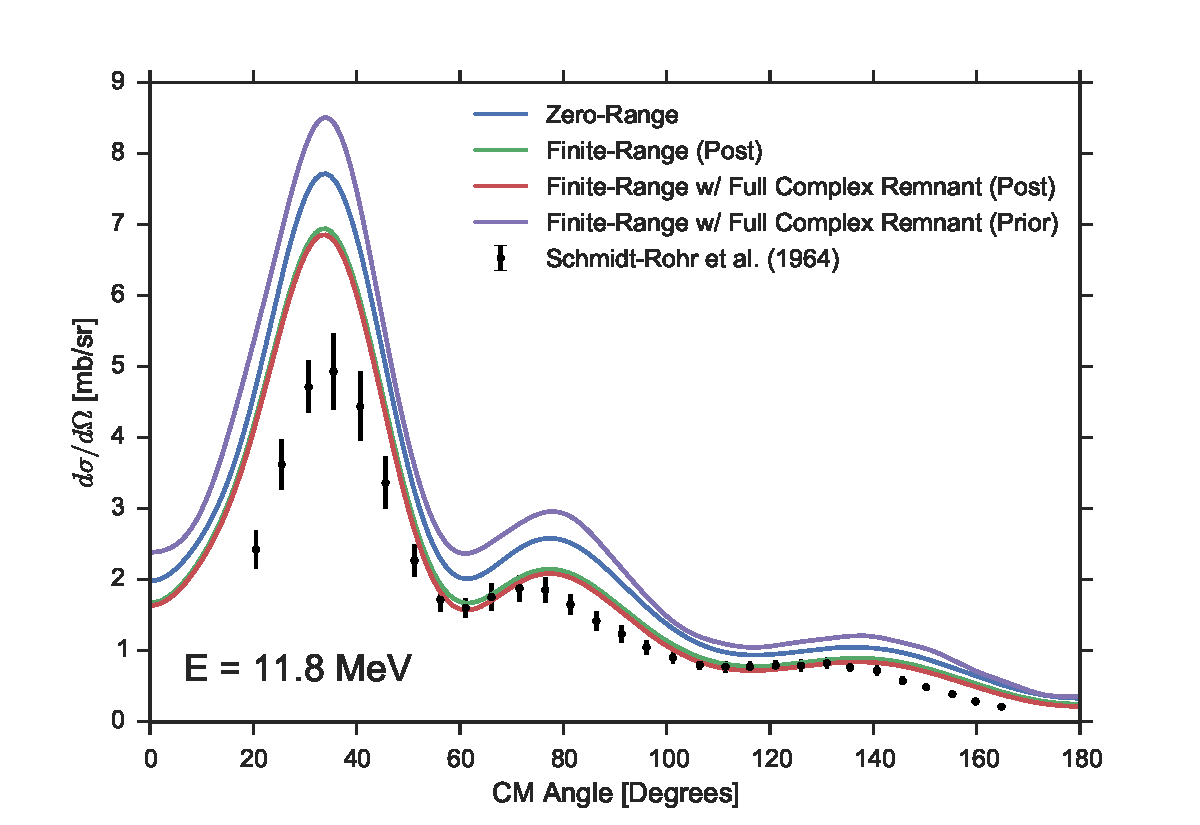
\includegraphics[width=\columnwidth]{{images/lowen.pdf}}
	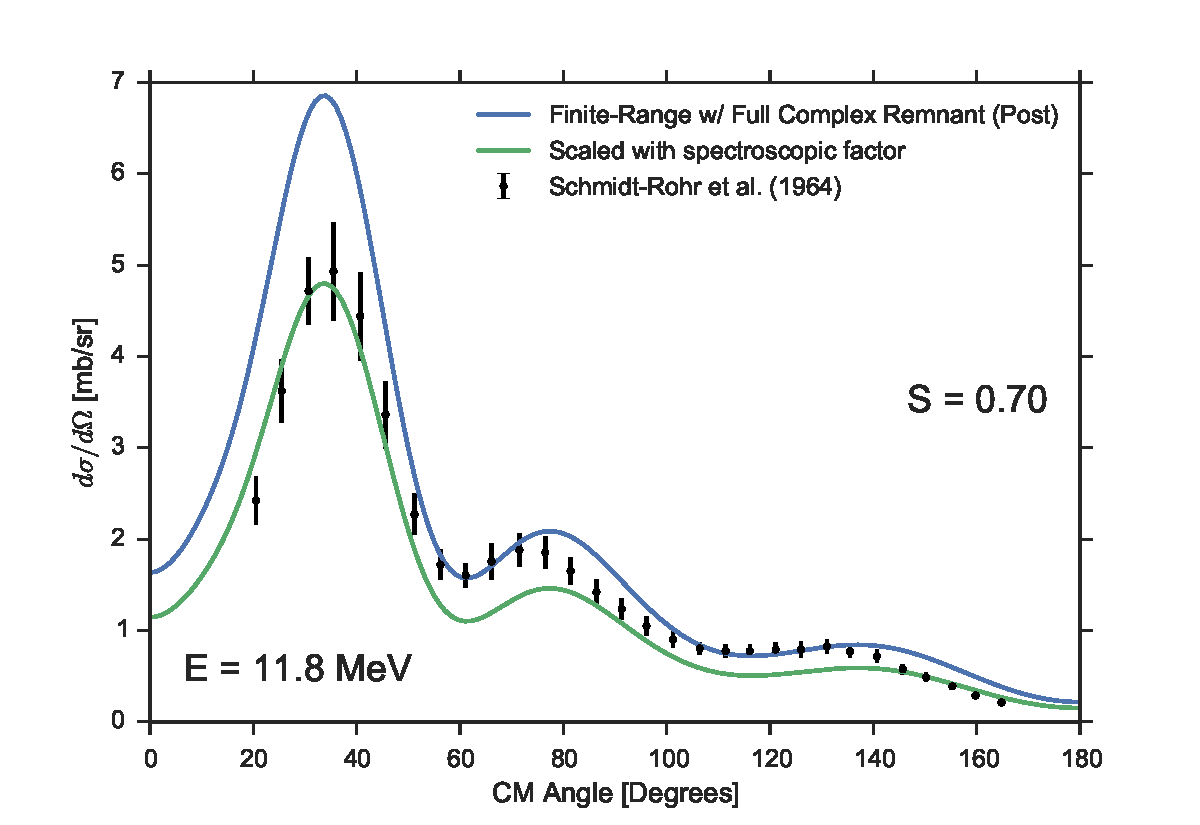
\includegraphics[width=\columnwidth]{{images/lowen_sfactor.pdf}}
	\caption{The left-hand graph shows the transfer cross sections at \SI{11.8}{MeV}. The black points represent experimental cross sections from Schmidt-Rohr et al. \cite{Schmidt-Rohr1964}. The right-hand plot shows a spectroscopic factor for the same data.}
	\label{fig:lowen}
\end{figure*}

\section{Low-energy results}

We then repeated this analysis at the lower energy of \SI{11.8}{MeV}. These results are shown in Fig.~\ref{fig:lowen}. The shape of this angular distribution is much different from the high-energy case. This is due to the effects of Coulomb repulsion, which are much more prominent at this lower energy. The output from \fresco at this energy agrees much better with experiment than in the high-energy case. The inconsistencies we do see are likely due to the fact that we could not find an optical potential valid for \nuc{41}{Ca}, so we used Koning and Delaroche's potential for \nuc{40}{Ca} instead, scaling the parameters that depended on proton separation energy appropriately.

As before, the post-form finite-range potentials are very similar to each other and somewhat different from the zero-range potential. Once again, the prior-form finite-range potential disagrees with the post-form results, likely due to numerical errors.

The right-hand plot in Fig.~\ref{fig:lowen} shows the finite-range post-form potential scaled with a spectroscopic factor of $S^\text{exp} = 0.70$ that was found visually, as before. The spectroscopic factor appears to be energy-dependent since this value is less than the value from the high-energy case. This energy dependence indicates that the higher-energy deuterons probe more deeply into the nucleus. This also seems to indicate that DWBA agrees more closely with experiment at a higher energy, though it is hard to be certain since the shape of our high-energy angular distribution was a bit off. It is also worth noting that both spectroscopic factors are less than one, as they must be.

\bibliography{hw3}

\end{document}